
\section{Data Collection and Filtering}
\subsection{BigData}
Recently, the ubiquitous availability of internet connections along with mobile technologies is generating a huge amount of data. This data is considered as BigData and it can be described as a large volume of complex data \cite{2}. Volume refers to the amount of data or quantities of data generated in a unit of time. Velocity refers to the speed at which data is generated and the speed at which data moves around. For example, social media messages going viral in seconds. Variety refers to the type of data that is generated. For example, as shown in \autoref{fig:bigdata}, data generated from mainframe source was less in volume and structured than today's data generated by different channels such as mobile messaging, social media, and internet.
\\
\begin{figure}[H]
	\centering
	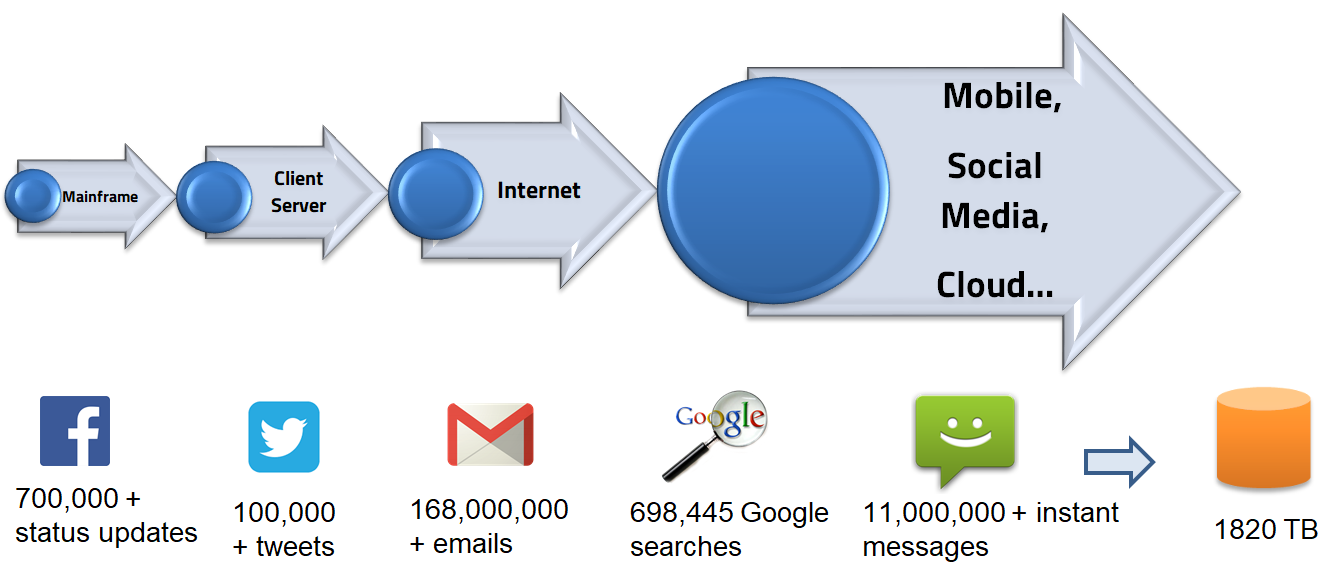
\includegraphics[width=0.7\linewidth]{bigdata}
	\caption{Growing Data Velocity per second}
	\label{fig:bigdata}
\end{figure}

\noindent Recommender systems can perform well based on a large amount of data. Big Data is a driving force behind recommendation engines.
To make this data useful, systems need to collect data, filter data in specific patterns from which we will get useful information. 

\subsection{Data Collection}

The data collection phase is a foundation of the accuracy of the recommendation engine. It is helpful to generate user profiles or models for making recommendations. To well construct a user profile, a recommendation engine relies on different types of inputs such as explicit feedback which is explicitly specified by a user to notify a user's interest in an item or providing implicit feedback by understanding user preferences from user's interaction with the system \cite{34}. 

\subsubsection{Explicit Data}
In explicit data collection, an application prompts the user through a user interface to provide feedback about the product in order to understand the user's preferences to improve the model. The user then interacts with the system by responding to these prompts. Explicit data is any information provided by a user explicitly or \textbf{knowingly} in the form of ratings, reviews, or comments. For example, below screen-shot shows that Netflix is collecting the data explicitly in the form of ratings given by the user to different movies. 
\\

\begin{figure}[H]
	\centering
	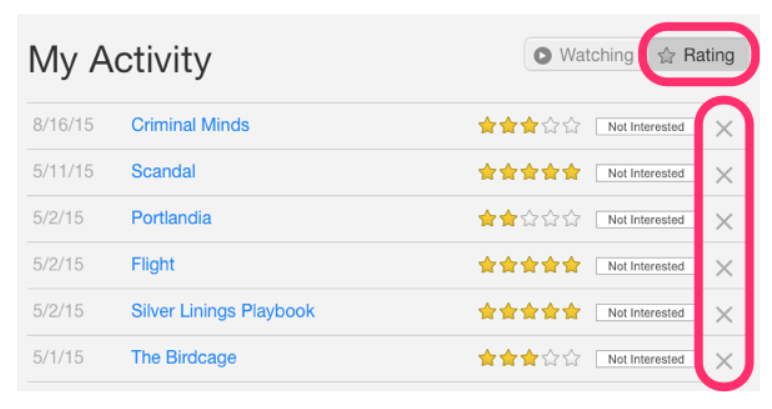
\includegraphics[width=0.9\linewidth]{explicit1}
	\caption{Explicit Data \cite{36}}
	\label{fig:explicit}
\end{figure}

\noindent Although explicit feedback requires more effort from the user, it is still reliable data as it does not require any extraction of preferences and it maintains transparency into the recommendation process \cite{35}.

\subsubsection{Implicit Data}

Implicit data implies to when a system attempts to understand more about user's preferences by monitoring interactions of a user such as browsing history, purchase history, button-clicks, links followed by a user. Implicit data is information provided by user \textbf{discretely} in the form of different interactions. For example, screenshot in \autoref{fig:implicit} shows that Amazon is collecting the data implicitly in the form of storing a user's order history.
\begin{figure}[H]
	\centering
	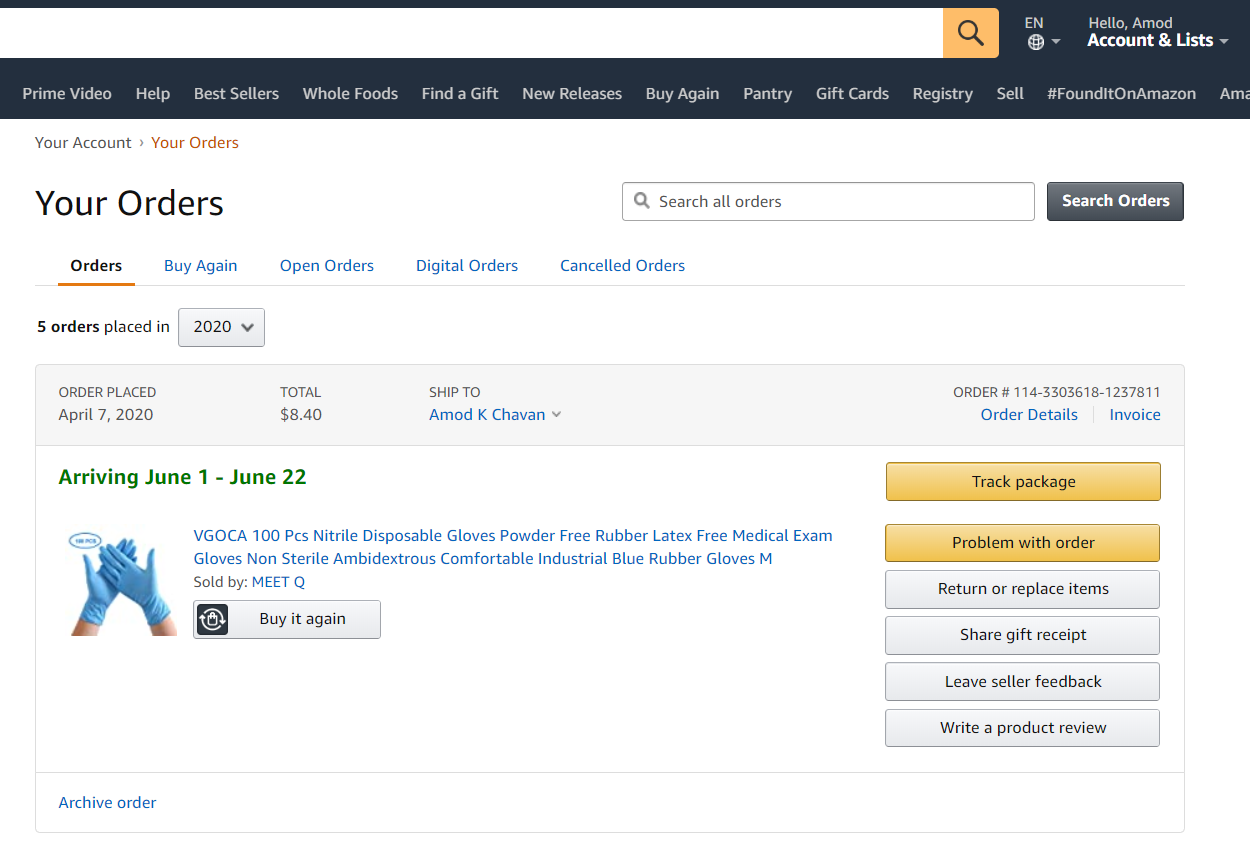
\includegraphics[width=0.9\linewidth]{order_history}
	\caption{Implicit Data}
	\label{fig:implicit}
\end{figure}

\noindent Based on a user's prior purchase, Amazon is recommending other products as shown in screen-shot \autoref{fig:implicit_reco}.

\begin{figure}[H]
	\centering
	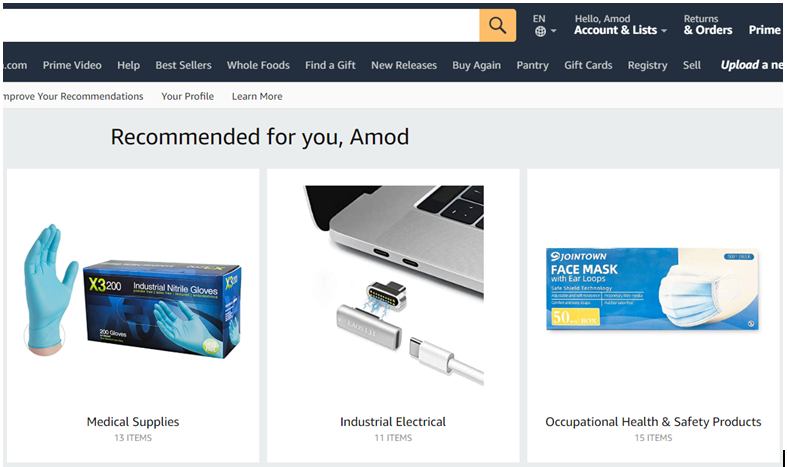
\includegraphics[width=0.9\linewidth]{reco_on_implicit_data}
	\caption{Recommendations based on Implicit Data}
	\label{fig:implicit_reco}
\end{figure}


\noindent Although implicit feedback does not require more effort from the user, it is less accurate. For example, a user of an e-commerce system purchase items as gifts for others. Those purchases and related activities do not necessarily communicate anything about the user’s tastes. A whole family may share a single account for purchases from e-commerce websites. In that case, input for the system will be an aggregation of all people's preferences.
\\
\\
Explicit and implicit data collection methods are used for building an online recommendation system. The work in this thesis is based on offline data. Different techniques are involved in offline data collection. \\
The information-gathering process involves many techniques such as web crawling, document processing, indexing and query processing. A crawler processes all URLs via techniques like breadth-first search and depth-first search and stores the web server's response for each URL. The documents retrieved are then processed in order for its meta-data and to remove any noisy data. Data indexing is then applied so that the retrieval and processing of extracted data are quicker.


\subsection{Information Filtering}

Information Filtering is associated with a data search. When a user requests information, it is treated as a query in the form of keywords and is applied on the indexed data. The objective of the query processor is to return the most relevant documents to the user.
\\
\noindent Filtering is a key component to retrieving adequate information per user preferences or user profile. User behavior is studied from past user-profiles activities which help to filter out any irrelevant data and provide relevant suggestions pertaining to current needs.
Recommendation process has three different phases as highlighted in \autoref{fig:reco_phases}. Data collection using different techniques such as explicit data and implicit data is known as the information collection phase. The different learning algorithms apply to the collected data to filter information. Applying algorithms to learn more about data is known as the learning phase.
Retrieving most relevant products or items by predicting what the user may prefer from filtered data is known as a recommendation or prediction phase.
\\
\begin{figure}[H]
	\centering
	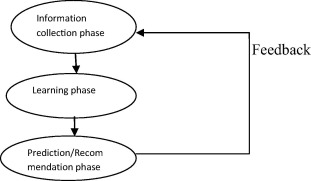
\includegraphics[width=0.7\linewidth]{reco_phases}
	\caption{Recommendation Phases \cite{33}}
	\label{fig:reco_phases}
\end{figure}
